%\listfiles
\documentclass[tg]{mdtuffs}
% um tipo específico de monografia pode ser informado como parâmetro opcional:
%\documentclass[tese]{mdtuffs}
% a opção `openright' pode ser usada para forçar inícios de capítulos
% em páginas ímpares
% \documentclass[openright]{mdtuffs}
% para gerar uma versão frente-e-verso, use a opção 'twoside':
% \documentclass[twoside]{mdtuffs}
%\usepackage{hyperref}	
%\usepackage{breakurl}
\usepackage[T1]{fontenc}        % pacote para conj. de caracteres correto
\usepackage{fix-cm}             % para funcionar corretamente o tamanho das fontes da capa
\usepackage{times, color,xcolor}% pacote para usar fonte Adobe Times e cores
\usepackage[utf8]{inputenc}     % pacote para acentuação
\usepackage{graphicx}           % pacote para importar figuras
\usepackage{caption}
\usepackage{float}              % para utilizar a opção H nas figuras.

%\usepackage[brazil]{babel}   
\usepackage{enumerate}
\usepackage{amsmath,latexsym,amssymb} %Pacotes matemáticos
\usepackage[%hidelinks%, 
            bookmarksopen=true,linktoc=none,colorlinks=true,
            linkcolor=black,citecolor=black,filecolor=magenta,urlcolor=blue,
            pdftitle={Geração procedural de biomas},
            pdfauthor={João Carlos Becker},
            pdfsubject={Projeto/Trabalho de Conclusão de Curso},
            pdfkeywords={Monografia, Modelo, LaTeX}
            ]{hyperref} %hidelinks disponível no pacote hyperref a partir da versão 2011-02-05  6.82a
%Nesse caso, hidelinks retira os retângulos em volta dos links das referências

%Definição de minha autoria pra funcionar as XML
%\def\lnl#1#2{{\scriptsize\bfseries #1}\hspace{#2em}}
\usepackage{setspace}
%---------------------------------------------------
% Definições dos XML
%---------------------------------------------------
\usepackage{verbatim}
\usepackage{listings}
%\usepackage[usenames,dvipsnames]{color}
	%\def\mlnl#1#2{{\scriptsize\bfseries #1}\hspace{#2em}}

%---------------------------------------------------
% Definições dos Algoritmos
%---------------------------------------------------
	\usepackage[portuguese,ruled,linesnumbered]{algorithm2e}
	\usepackage{etoolbox}
	\makeatletter
	\patchcmd{\@algocf@start}{%
		\begin{lrbox}{\algocf@algobox}%
	}{%
	  \rule{0.\textwidth}{\z@}%
	  \begin{lrbox}{\algocf@algobox}%
	  \begin{minipage}{1.\textwidth}%
	}{}{}
	\patchcmd{\@algocf@finish}{%
	  \end{lrbox}%
	}{%
	  \end{minipage}%-----------------------------------------------------------Tem erro de sintaxe aqui
	  \end{lrbox}%
	}{}{}
	\makeatother

	\SetAlFnt{\tt}
	
	\SetKwFunction{FRecurs}{FnRecursive}%
%-------------------------------------------------

     
\sloppy
%%Margens conforme MDT 1ª edição, arrumar diretamente no mdtuffs.cls para funcionar a opção twoside *PENDENTE*
\usepackage[inner=30mm,outer=20mm,top=30mm,bottom=20mm]{geometry} 

%==============================================================================
% Se o pacote hyperref foi carregado a linha abaixo corrige um bug na hora
% de montar o sumário da lista de figuras e tabelas
% Se o pacote não foi carregado, comentar a linha %
%==============================================================================

%%=============================================================================
%% Trampa para corrigir o bug do hyperref que redefine o caption das figuras e das
%% tabelas, n�o colocando o nome ``Figura'' antes do n�mero do mesmo na lista
%%=============================================================================

\makeatletter

\long\def\@caption#1[#2]#3{%
  \expandafter\ifx\csname if@capstart\expandafter\endcsname
                  \csname iftrue\endcsname
    \global\let\@currentHref\hc@currentHref
  \else
    \hyper@makecurrent{\@captype}%
  \fi
  \@ifundefined{NR@gettitle}{%
    \def\@currentlabelname{#2}%
  }{%
    \NR@gettitle{#2}%
  }%
  \par\addcontentsline{\csname ext@#1\endcsname}{#1}{%
    \protect\numberline{\csname fnum@#1\endcsname ~-- }{\ignorespaces #2}%
  }%
  \begingroup
    \@parboxrestore
    \if@minipage
      \@setminipage
    \fi
    \normalsize
    \expandafter\ifx\csname if@capstart\expandafter\endcsname
                    \csname iftrue\endcsname
      \global\@capstartfalse
      \@makecaption{\csname fnum@#1\endcsname}{\ignorespaces#3}%
    \else
      \@makecaption{\csname fnum@#1\endcsname}{%
        \ignorespaces
        \ifHy@nesting
          \expandafter\hyper@@anchor\expandafter{\@currentHref}{#3}%
        \else
          \Hy@raisedlink{%
            \expandafter\hyper@@anchor\expandafter{%
              \@currentHref
            }{\relax}%
          }%
          #3%
        \fi
      }%
    \fi
    \par
  \endgroup
}

\makeatother

%==============================================================================
% Identificação do trabalho
%==============================================================================
\title{Geração procedural de biomas}

\author{Becker}{João Carlos}
%Descomentar se for uma "autora"
%\autoratrue

\course{Curso de Ciência da Computação}
\altcourse{Curso de Ciência da Computação}

%não usado por enquanto
\institute{Ciência da Computação}
\degree{Bacharel em Ciência da Computação}

% Número do TG (verificar na secretaria do curso)
% Para mestrado deixar sem opção dentro do {}
\trabalhoNumero{}

%Orientador
\advisor[Prof.]{Dr.}{Wuerges}{Emílio}
%Se for uma ``orientadora'' descomentar a linha baixo
%\orientadoratrue

%Co orientador, comentar se não existir
%\coadvisor[Prof.]{Drª.}{Pereira}{Maria Regina}
%\coorientadoratrue %Se for uma ``Co-Orientadora''

%Avaliadores (Banca)
\committee[Dr.]{de Mello}{Braulio Adriano}{UFFS}
\committee[Dr.]{Bins Filho}{José Carlos}{UFFS}

% a data deve ser a da defesa; se nao especificada, são gerados
% mes e ano correntes
\date{11}{Dezembro}{2017}

%Palavras chave
%\keyword{Dissertação} 
%\keyword{Modelo}
%\keyword{LaTeX}

%%=============================================================================
%% Início do documento
%%=============================================================================
\begin{document}

%%=============================================================================
%% Capa e folha de rosto
%%=============================================================================
\maketitle

%%=============================================================================
%% Catalogação e Folha de aprovação
%%=============================================================================
%\clearpage
%Somente para TCC 2: Está página deve ser substituida pela ficha de catalogação antes de sua entrega na biblioteca. 
%Somente obrigatório para dissertação, para TG, remover as linhas	77	%
%Como a CIP vai ser impressa atrás da página de rosto, as margens inner e outer	
%devem ser invertidas.
%\newgeometry{inner=20mm,outer=30mm,top=30mm,bottom=20mm}	
%\makeCIP{email@email.com} %email do autor		
%\restoregeometry

%Se for usar a catalogação gerada pelo gerador do site da biblioteca comentar as linhas
%acima e utilizar o comando abaixo
%\includeCIP{CIP.pdf}

%folha de aprovação

%IMPORTANTE: Esta folha deverá ser impressa e assinada pela banca e depois digitalizada e inserida no arquivo final para entrega no repositório institucional.
\makeapprove

%%=============================================================================
%% Dedicatória (opcional)
%%=============================================================================
%\clearpage
%\begin{flushright}
%\begin{onehalfspacing}
%\mbox{}\vfill

%{Texto da dedicatória ......}

%\end{onehalfspacing}
%\end{flushright}

%%=============================================================================
%% Agradecimentos (opcional)
%%=============================================================================
%\clearpage
%{
%\centering
%\textbf{AGRADECIMENTOS}\\
%}
%\vspace{1.5cm}
%\begin{onehalfspacing}

%Texto de agradecimento. 

%\end{onehalfspacing}


%%=============================================================================
%% Epígrafe (opcional)
%%=============================================================================
%\clearpage
%\begin{flushright}
%\mbox{}\vfill
%{\sffamily\itshape
%``Frase da epígrafe'' \\ }
%--- \textsc{Autor da frase}
%\end{flushright}


%%=============================================================================
%% Resumo
%%=============================================================================
\begin{abstract}
    Os jogos digitais estão cada vez melhores e exigindo mais complexidade para
    os mesmos, trazendo mais conteúdo agregado. O tempo para produzir este conteúdo
    demanda muito esforço de trabalho. Com a intenção de auxilar nestas
    dificuldades, a geração procedural de conteúdo consegue gerar gráficos com pouca
    ou nenhum esforço do usuário. Neste trabalho será avaliado algumas características
    de relevo, como planícies e cordilheiras, e implementar um algoritmo não 
    assistido que forme proceduralmente o relevo dessas características, na ocorrência
    de fronteiras de biomas com relevo distintos, a mesma será contínua.
    No final será feito um julgamento visual sobre os resultados, comparando com 
    características encontradas na natureza e outros jogos. O tamanho do mapa
    deve ser pseudo infinito e carregar apenas regiões próximas da câmera.
    \keyword{Geração procedural de conteúdo}
    \keyword{Mapas de altura}
    \keyword{jogos 3D}
\end{abstract}










%%=============================================================================
%% Abstract
%%=============================================================================
% resumo na outra língua
% como parametros devem ser passados o titulo, o nome do curso,
% as palavras-chave na outra língua, separadas por vírgulas, o mês em inglês
%o a sigla do dia em inglês: st, nd, th ...
\begin{englishabstract}
{Biome procedural generation}
{Bachelor of Computer Science}
{Procedural Content Generation, Height maps, 3D games}
{July}
{fr}
Digital games are always improving, increasing in complexity and using more and more content.
Time spent to produce this content requires a lot of human effort.
With the intent of coping with this challenge, procedural generation of content can produce graphical content with little or no human intervention.
In this work we will analyze features of the terrain, such as plains and mountain ranges, and 
implement an unattended algorithm that produces a world with many regions, each containing terrain with one these features, which we call biomes. 
The border of different biomes must be continuous. 
The size of the world will be pseudo-infinite, but only regions close to the camera will be loaded in memory.
To evaluate our algorithm, we will judge the results visually, comparing them with either nature or games.

\end{englishabstract}

%% Lista de Ilustrações (opc)
%% Lista de Símbolos (opc)
%% Lista de Anexos e Apêndices (opc)

%%=============================================================================
%% Lista de figuras (comentar se não houver)
%%=============================================================================
\listoffigures

%%=============================================================================
%% Lista de tabelas (comentar se não houver)
%%=============================================================================
%\listoftables

%%=============================================================================
%% Lista de Apêndices (comentar se não houver)
%%=============================================================================
%\listofappendix

%%=============================================================================
%% Lista de Anexos (comentar se não houver)
%%=============================================================================
%\listofannex

%%=============================================================================
%% Lista de abreviaturas e siglas
%%=============================================================================
% O parametro deve ser a abreviatura mais longa
\begin{listofabbrv}{ESA}
\item [GLSL] \textit{OpenGL Shading Language}
\item [ESA] \textit{Entertainment Software Association}
\item [GDP] \textit{Gross domestic product}
\item [PCG] \textit{Procedural Content Generation}
    
%   \item [BNF] \textit{Backus-Naur Form}
%  \item [UbiComp] Computação Ubíqua
\end{listofabbrv}


%%=============================================================================
%% Lista de simbolos (opcional)
%%=============================================================================
%Simbolos devem aparecer conforme a ordem em que aparecem no texto
% o parametro deve ser o símbolo mais longo
%\begin{listofsymbols}{teste}
 % \item [$\varnothing$] vazio
 % \item [$\Gamma$]  Gama
 % \item [$\forall$] Para todo
%\end{listofsymbols}

%%=============================================================================
%% Sumário
%%=============================================================================
\tableofcontents


%%=============================================================================
%% Início da monografia
%%=============================================================================
\setlength{\baselineskip}{1.5\baselineskip}

%Adiciona cada capitulo
\begin{frame}{Problemática}
    \begin{itemize} \setlength\itemsep{1em}
        \item Os jogos digitais estão cada vez melhores e exigindo mais
        complexidade para os mesmos, trazendo mais conteúdo agregado.
        \item O tempo para produzir este conteúdo demanda muito esforço de trabalho.
    \end{itemize}
\end{frame}


%\begin{frame}{Introdução}
%    
%\end{frame}

\begin{frame}{Objetivos}
    \begin{itemize}
        \item Objetivo Geral
        \begin{itemize}
            \item Este projeto tem como objetivo gerar mapas de tamanho pseudo-infinitos, com 
            relevo gerado proceduralmente usando ruído 
            de Perlin, de maneira não assistida, os mapas de altura devem representar o 
            relevo de pelo menos dois biomas arbitrários com fronteiras contínuas.
        \end{itemize}
        \item Objetivos Específicos
        \begin{itemize}
            \item Implementar malhas da superfície com tamanho pseudo-infinito;
            \item Selecionar biomas, e as características dos mesmos a ser representadas;
            \item Construir algoritmo para manipular ruído de Perlin e gerar características
                selecionadas do bioma;
            \item Gerar divisões entre biomas sobre a malha de regiões;
            \item Implementar fronteiras contínuas entre biomas;
            \item Comparar resultado com cenários de jogos.
        \end{itemize}
    \end{itemize}
\end{frame}
%duvida 1: qual melhor pessoa para usar em frazes
%   nessa etapa precisamos (ingles)
%   nessa etapa é preciso
%   nessa etapa precisei
%   nessa etapa foi necessário       usar essa

%Conjunto de equações, recomendação do emílio
%\begin{align}
%    A \in Z^{2} \\
%    mix(A, B, c) &= (1-c) * A + c*B \\
%    mix(A, B, c) &= (1-c) * A + c*B \\
%\end{align}

\chapter{Implementação}

%Essa seção não é muito relevante para o resultado final, não sei se escrevo ela
\section{Configuração do Ambiente}

%Mover para fundamentação teórica
\subsection{Usando os Buffers do OpenGL e GLSL}

\subsubsection{Descrição dos vértices}
Um vértice $v$ é um conjunto de informações relacionadas a alguma unidade, %DEBUG: trocar o termo unidade
a informação necessária para este projeto é posição no espaço, então cada vértice
vai possuir uma posição notada por $v.pos$, e $v.pos$ é composto por 
$\{x, y, z\} \in \mathbb{Q}^3$. Um segundo dado será usado, a cor, vai ser uma 
informação auxiliar, usada para melhor vizialização dos resultados, 
representada por $\{r, g, b \in \mathbb{Q}:0 \leq r, g, b \leq 1\}$ onde cada um desses
vai referir a proporção de vermelho, verde e azul respectivamente.

\subsubsection{Implementação do sistema de Navegação}

\section{\textit{Terrain chunk}}
Representando um fragmento do terreno, o objeto \textit{Terrain chunk} é responsavel
por gerar uma malha para o terreno com $k^2$ vértices, o construtor pode receber 
a seguinte tupla para inicialização: 
$terrainChunk(seed, \Delta{v}, k, x_{s}, z_{s}, b, l)$
%referenciar as fatias do fernando
\begin{itemize}
    \item $seed \in \mathbb{N}$ representa a semente para começar o motor de números
    pseudo-aleatórios;
    \item $\Delta{v} \in \mathbb{Q}:0 < \Delta{v} < l/2$ é a distância entre vértices adjeacentes na
    projeção do plano $X \times Z$;
    \item $k \in \mathbb{N}>4$ é a quantidade de vértices em cada coluna ou 
    linha, a malha tem $k^2$ vértices;
    \item $x_{s} \in \mathbb{Q}:$ é o valor inicial no eixo $X$;
    \item $z_{s} \in \mathbb{Q}:$ é o valor inicial no eixo $Z$;
    \item $b \in \mathbb{N}>4:$ a área da região de cada bioma vai ser $b^2$;
    \item $l \in \mathbb{N}:1 < l < b/2$ distância para fronteira entre biomas ser interpolada.
\end{itemize}


Em cada execução da iplementação os valores que podem mudar de uma chunk para 
outra são apenas $x_{s}$ e $z_{s}$. Uma maneira de conseguir gerar terreno sobre demanda
é usando a localização da camera $(x_{c}, y_{c}, z_{c})$, quando ela se
aproxima de alguma borda da chunk atual
uma \textit{thread} é acionada pedidndo para calcular uma nova chunk, com os parâmetros
$terrainChunk(seed, \Delta{v}, k, x_{c}/\Delta{v} - k/2, z_{c}/\Delta{v} - k/2, b, l)$, assim que ela %debug: atualizar fórmula
estiver calculada a mesma começa a ser renderizada, substituindo a chunk anterior.
Antes de renderizar alguma chunk é necessário fazer uma translação com o vetor direção 
$(x_{s} * \Delta{v}, 0.0, z_{s} * \Delta{v})$, já que internamente cada chunk vai 
da posição $(0, 0)$ até $(\Delta{v}*(k-1), \Delta{v}*(k-1))$, mas representando a área 
no mundo $(x_{s}, z_{s})$ até $(x_{s} + \Delta{v}*(k-1), z_{s} + \Delta{v}*(k-1))$

\section{Criando Malha de Triângulos}
A maneira que um jogo renderiza seu terreno no final das contas é sobre uma
malha, uma malha é um conjunto de vértices que podem representar fragmentos
de uma superfície do terreno.

Para representar um segmento de plano precisamos de pelo menos $3$ vértices, 
já que com dois podemos apenas representar segmentos de retas. Um plano precisar
ter um mesmo vetor normal para todo o plano.

A malha segue pelo plano $X \times Z$, e cada vértice do plano vai ter uma altura
$y$ definida mais tarde por ruído. Se quisermos que o conjunto de pontos pertença
ao memos segmento de plano precisamos que os quatro pontos respeitem a mesma
equação do plano.%colocar referêrencia da malha de triângulos

Se usarmos como plano $4$ pontos em $\mathbb{Q}^3$
\begin{equation}\label{comp_sign_inter_sem_peso_aux}
    P = \{p_{0}(0, y_{0}, 0), p_{1}(0, y_{1}, 1), p_{2}(1, y_{2}, 0), p_{3}(1, y_{3}, 1)\}
\end{equation}
Para montar a equação do plano temos $\{y_{0}, y_{1}, y_{2}\}$ como valores livres e $y_{3}$
vai depender dos valores de $\{p_{0}, p_{1}, p_{2}\}, x_{3} e z_{3}$

%Aqui vai o cálculo da equação do plano ou do vetor normal para mostrar o que
%acabei de afirmar acima
%Calculando o vetor normal associado ao plano formado por $\{v0, v1, v2\}$
%$v0v1 = (0, y1-y0, 1)$
%$v0v2 = (1, y2-y0, 0)$

mas não é isso o objetivo, já que o ruído pode retornar valores para $y_{3}$
que não respeitem a equação do plano queremos que todos os pontos tenha valores de $y$
livres, portanto, será uma malha de triângulos. Então pro conjunto de vértices
acima temos dois triângulos associados:
$T_{1} = \{p_{0}, p_{1}, p_{2}\}, T_{2} = \{p_{3}, p_{1}, p_{2}\}$, que podem ser
vizualizados na figura \ref{fig:t1t2}. 
Desta maneira temos todos os pontos com $y$ livre.

\begin{figure}[H]
    \centering
    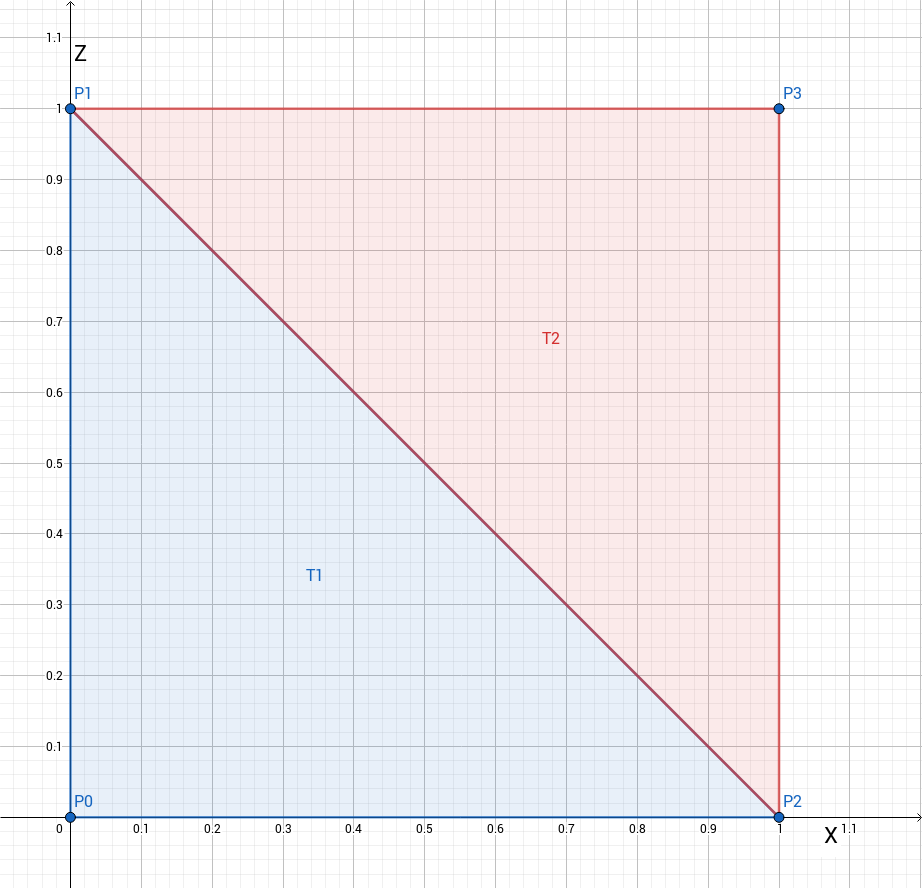
\includegraphics[width=0.5\textwidth]{figuras/t1t2.png}
    \caption{$T_{1}$ e $T_{2}$ projetados em $X \times Z$}
    \label{fig:t1t2}
\end{figure}


Então para montar um grid renderizavel usamos o algoritmo \ref{alg:genVectors}
$V$ é a estrutura que armazena os vértices, de $v_{0}$ até $v_{k^2-1}$ 
$E$ é a estrutura que armazena os índices, já que o \textit{OpenGL} precisa
saber a ordem de desenhar cada triângulo e quais vértices fazem parte dele, 
cada elemento de $e_{i} \in \mathbb{N}$ e a estrutura vai de $e_{0}$ até $e_{(k-1)^2 * 6 - 1}$.

A função \textit{hEvaluation}, vamos comentar mais adiante, ela retorna uma estrutura
com a altura e cor para algum ponto $(x, z)$.
 
\begin{algorithm}[H]\label{alg:genVectors}
    $|V| = k^2$\;
    \For{$i=0$ \KwTo $k-1$}{
        \For{$j=0$ \KwTo $k-1$}{
            $v_{i*k + j}.pos = (\Delta_{v} * i, hEvaluation(\Delta_{v} * i, \Delta_{v} * j).h, \Delta{v} * j)$\;
            $v_{i*k + j}.cor = hEvaluation(\Delta_{v} * i, \Delta_{v} * j).c$
        }
    }
    
    \For{$i=0$ \KwTo $k-2$}{
        \For{$j=0$ \KwTo $k-2$}{
            //posições em $V$ do primeio triângulo\;
            $E.$pushBack$(i*k +j)$\;
            $E.$pushBack$(i*k +j+1)$\;
            $E.$pushBack$((i+1)*k +j)$\;
            //posições em $V$ do segundo triângulo\;
            $E.$pushBack$((i+1)*k +j+1)$\;
            $E.$pushBack$(i*k +j+1)$\;
            $E.$pushBack$((i+1)*k +j)$\;
        }
    }
    \caption{Construção da coleção de vértices e índices.}
\end{algorithm}

\begin{figure}[H]
    \begin{figure}[H]
        \centering
        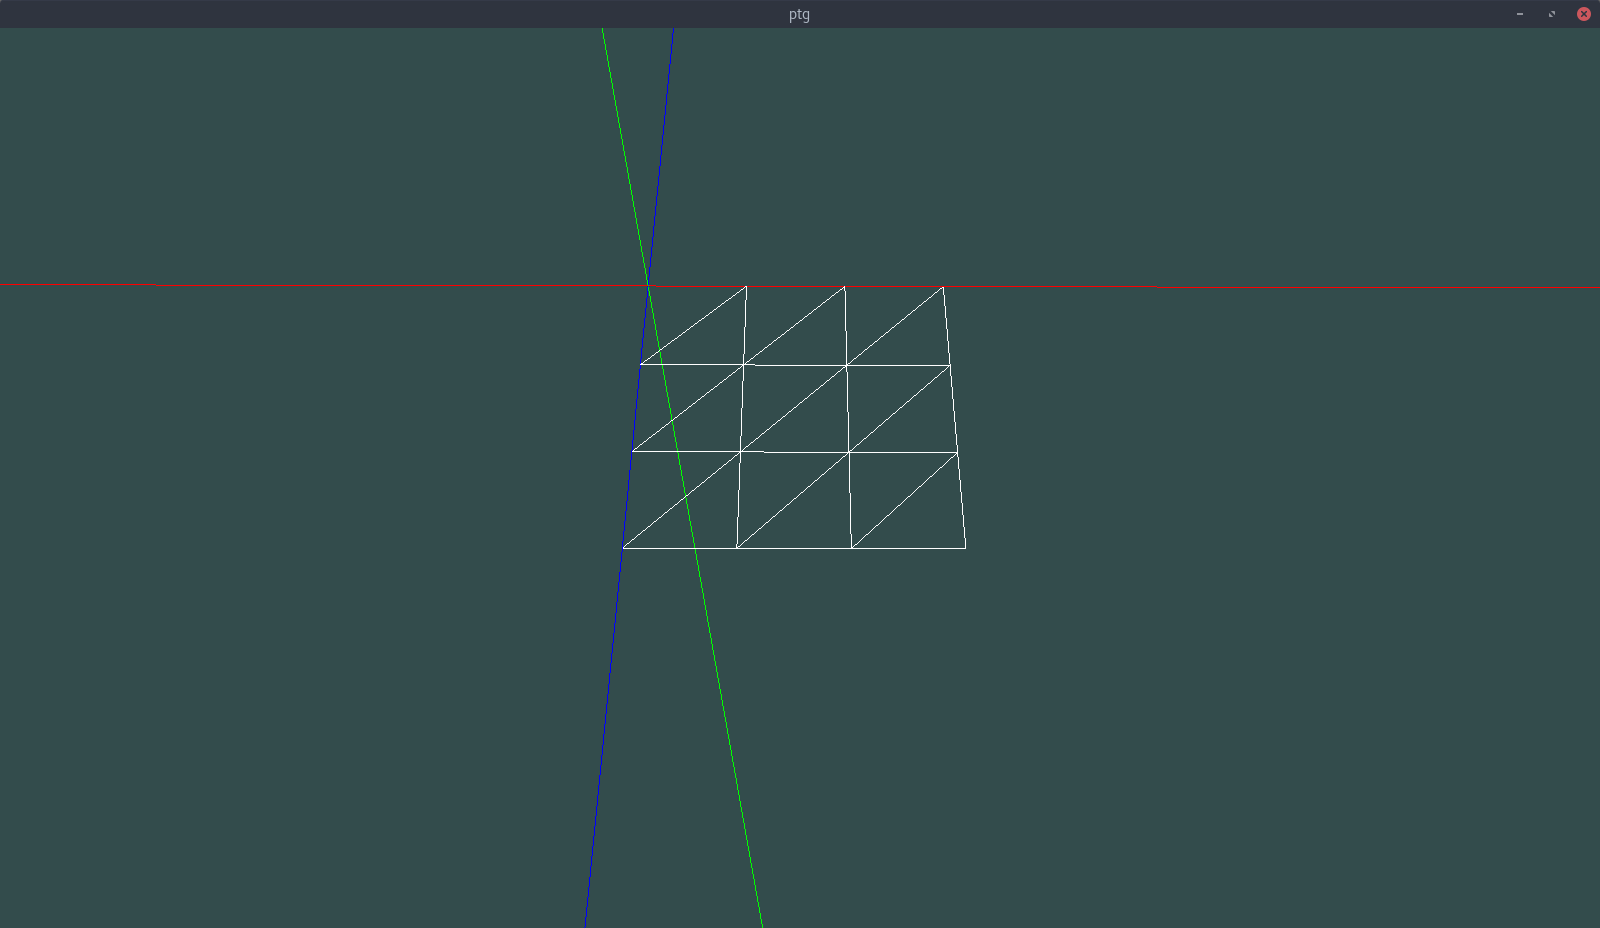
\includegraphics[width=0.2\textwidth]{figuras/k4d5.png}
        \caption{$T_{1}$ e $T_{2}$ projetados em $X \times Z$}
        \label{fig:k4d5}
    \end{figure}

    \begin{figure}[H]
        \centering
        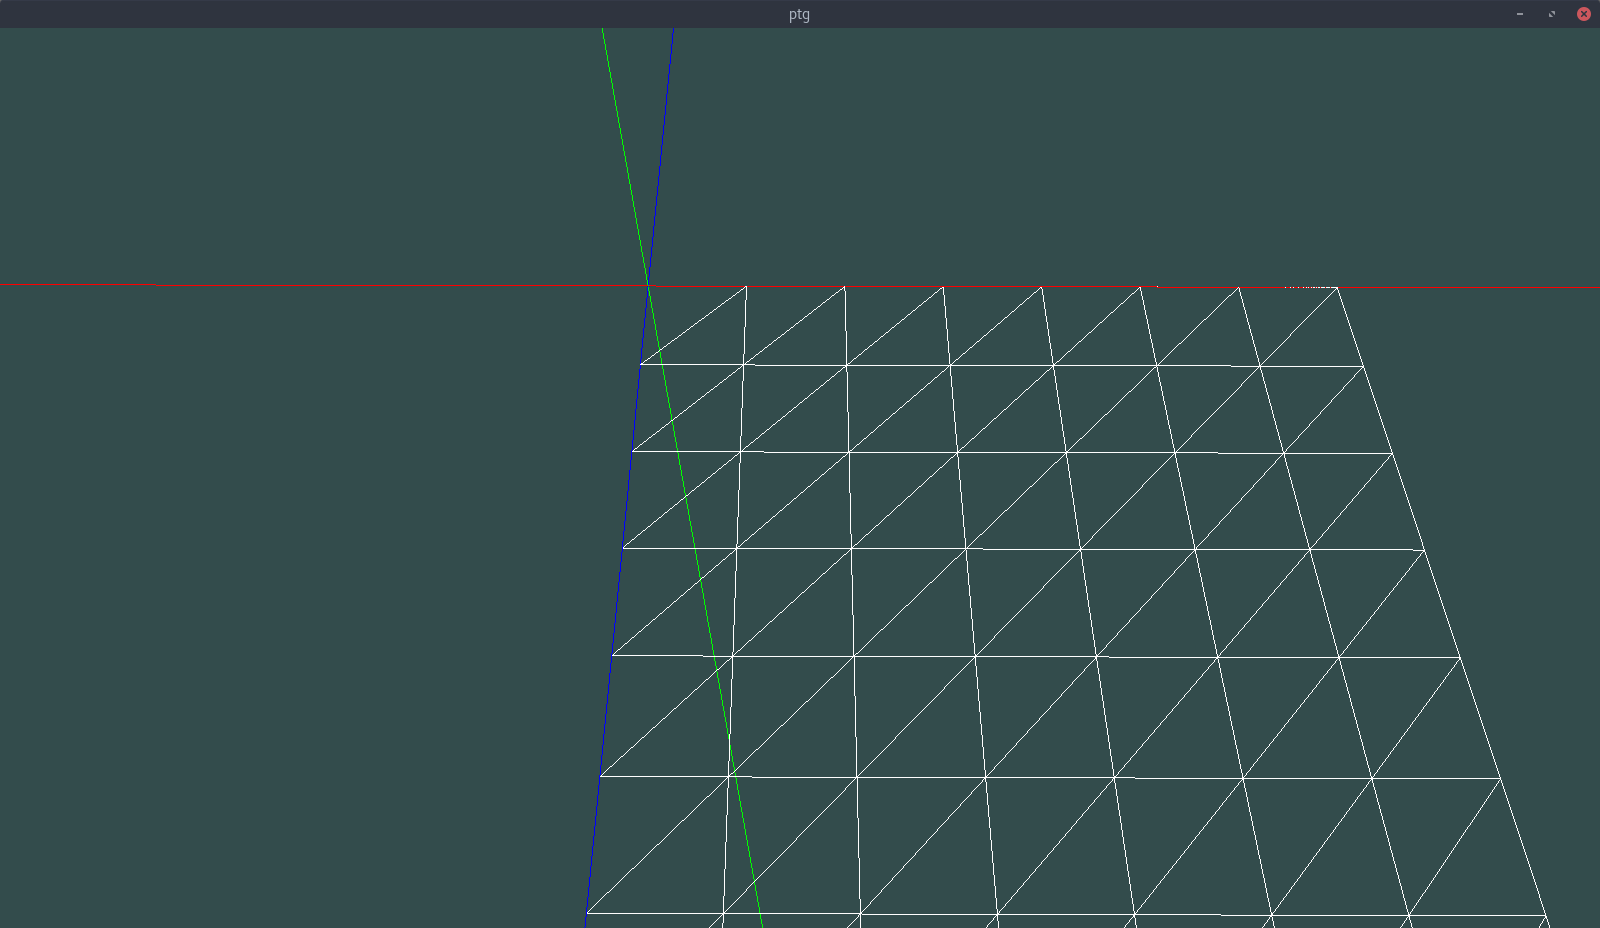
\includegraphics[width=0.2\textwidth]{figuras/k8d5.png}
        \caption{$T_{1}$ e $T_{2}$ projetados em $X \times Z$}
        \label{fig:k8d5}
    \end{figure}

    \begin{figure}[H]
        \centering
        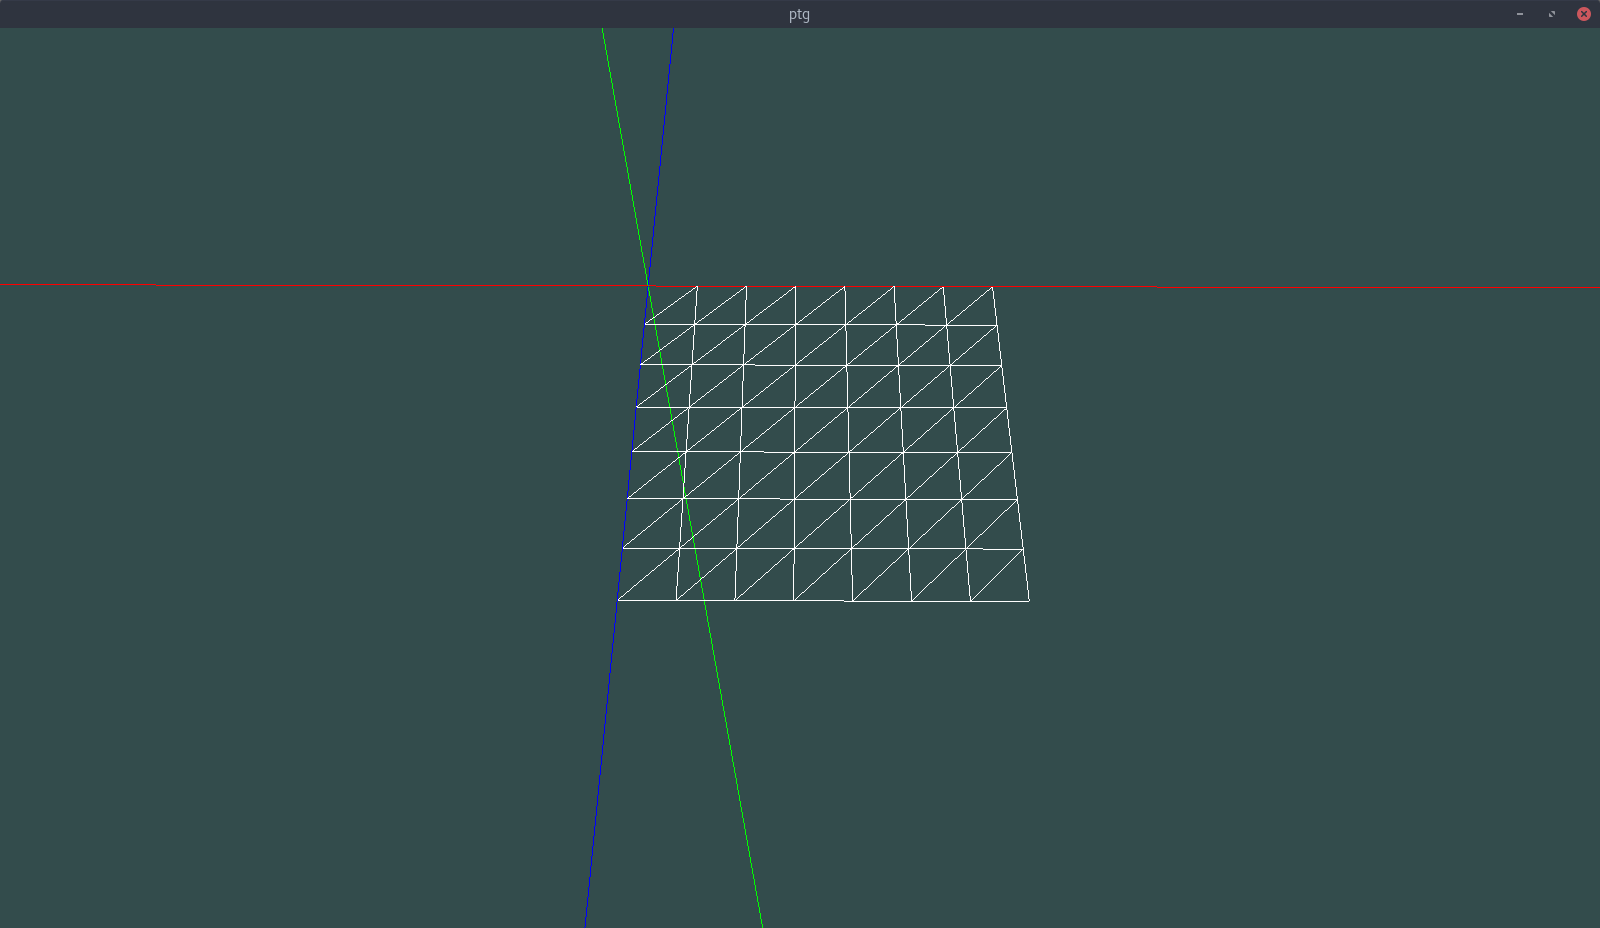
\includegraphics[width=0.2\textwidth]{figuras/k8d25.png}
        \caption{$T_{1}$ e $T_{2}$ projetados em $X \times Z$}
        \label{fig:k8d25}
    \end{figure}
    
\end{figure}




\section{Aplicando Ruído de Perlin nos Vértices}

\subsection{Manipulando ruído para criar Biomas}
\subsubsection{PLAINS}

\begin{figure}[H]
    \centering
    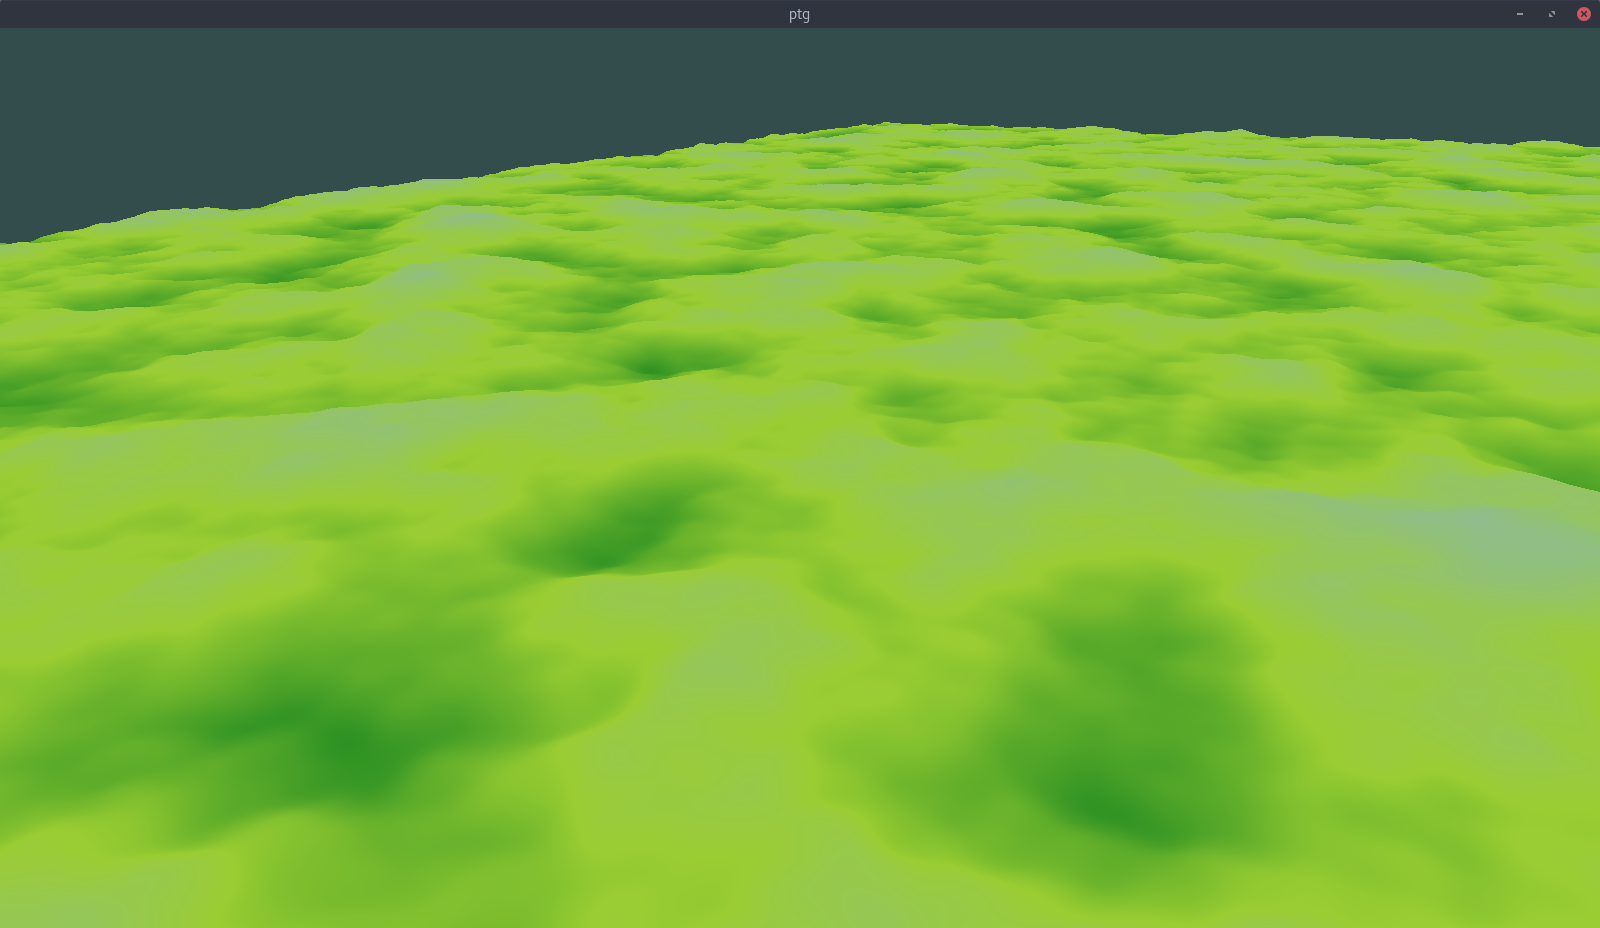
\includegraphics[width=0.5\textwidth]{figuras/bssPlains.png}
    \caption{Consumo}
    \label{fig:bssPlains}
\end{figure}

\subsubsection{MONTAINS}


\begin{figure}[H]
    \centering
    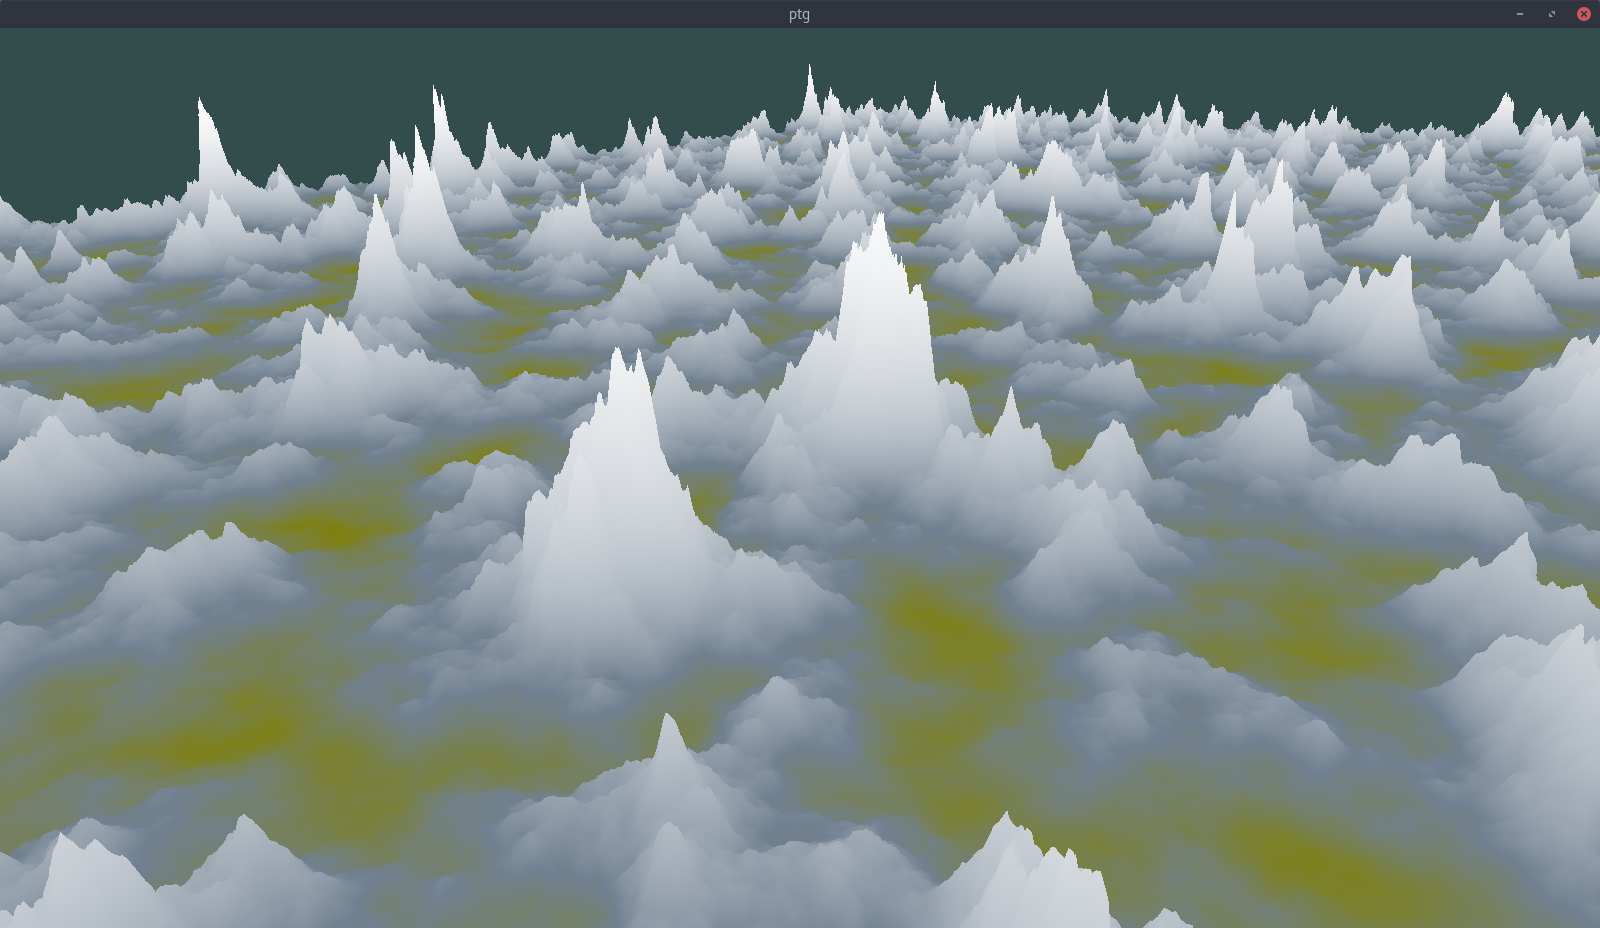
\includegraphics[width=0.5\textwidth]{figuras/bssMontains.png}
    \caption{Consumo}
    \label{fig:bssMontains}
\end{figure}

\subsubsection{VALLEY}


\begin{figure}[H]
    \centering
    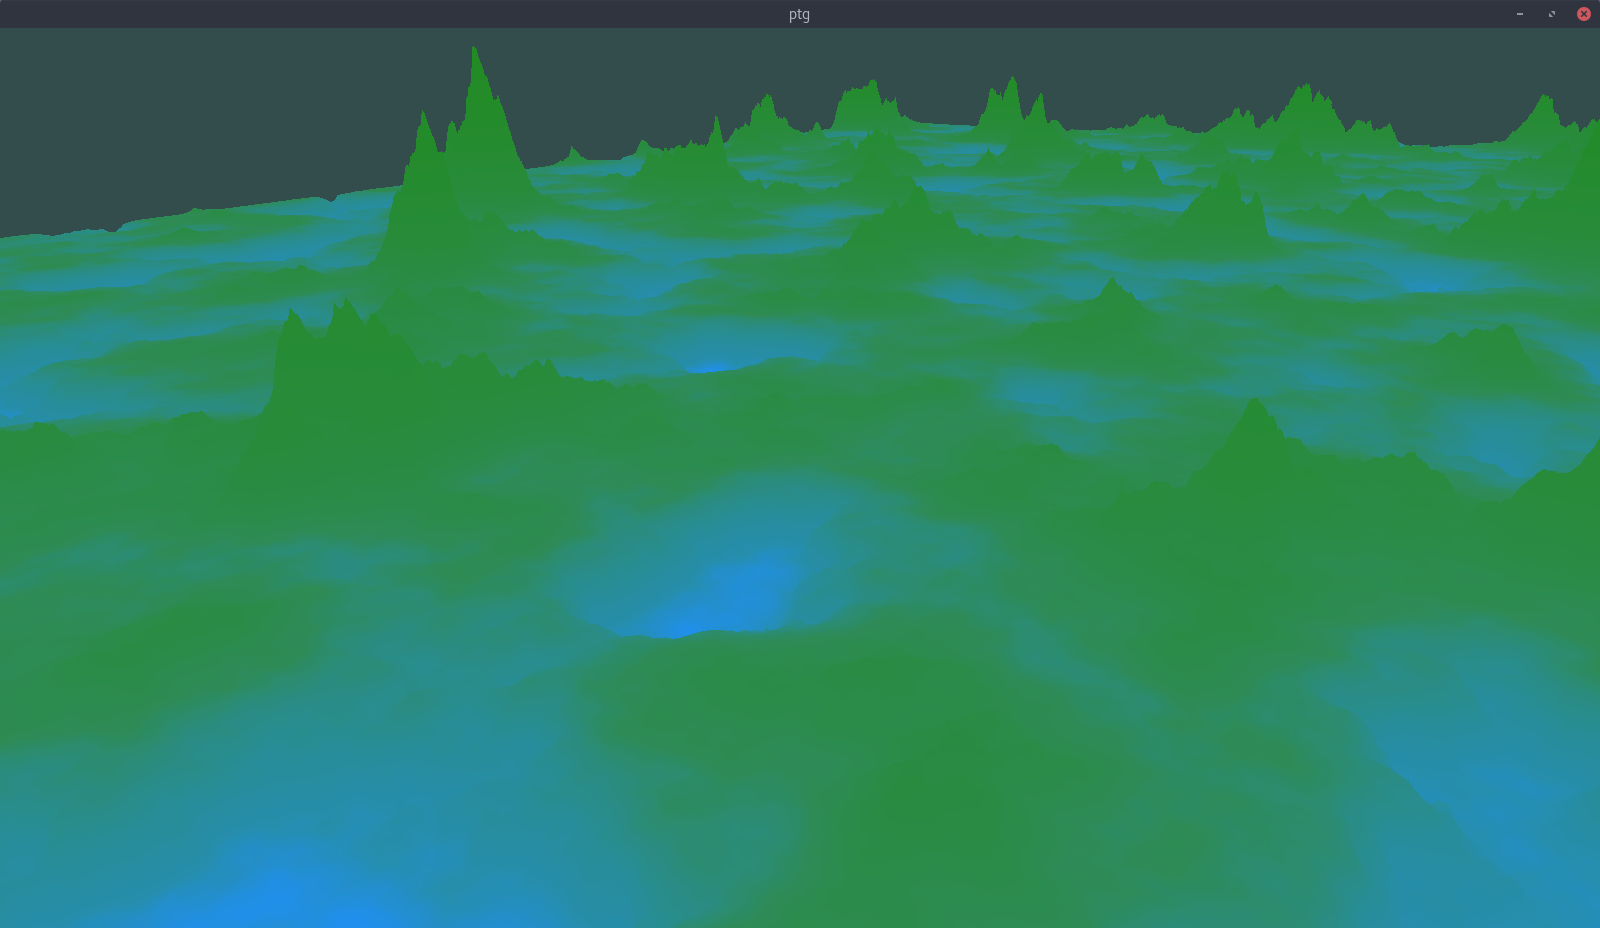
\includegraphics[width=0.5\textwidth]{figuras/bssValley.png}
    \caption{Consumo}
    \label{fig:bssValley}
\end{figure}

\subsubsection{DESERT}


\begin{figure}[H]
    \centering
    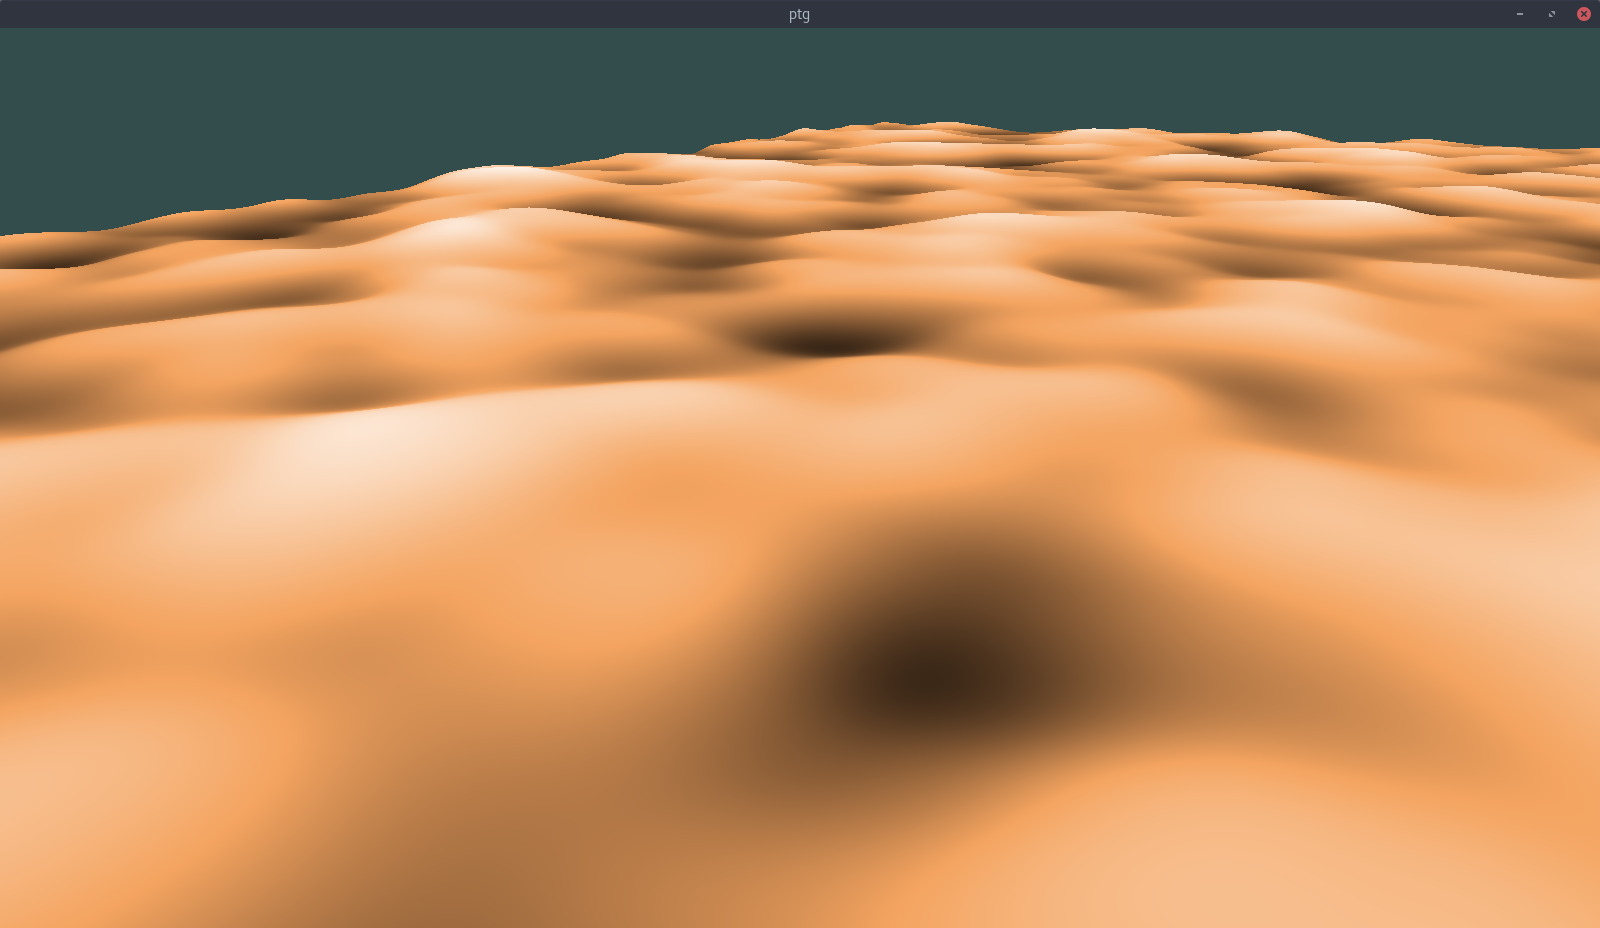
\includegraphics[width=0.5\textwidth]{figuras/bssDesert.png}
    \caption{Consumo}
    \label{fig:bssDesert}
\end{figure}

\subsubsection{CANYONS}


\begin{figure}[H]
    \centering
    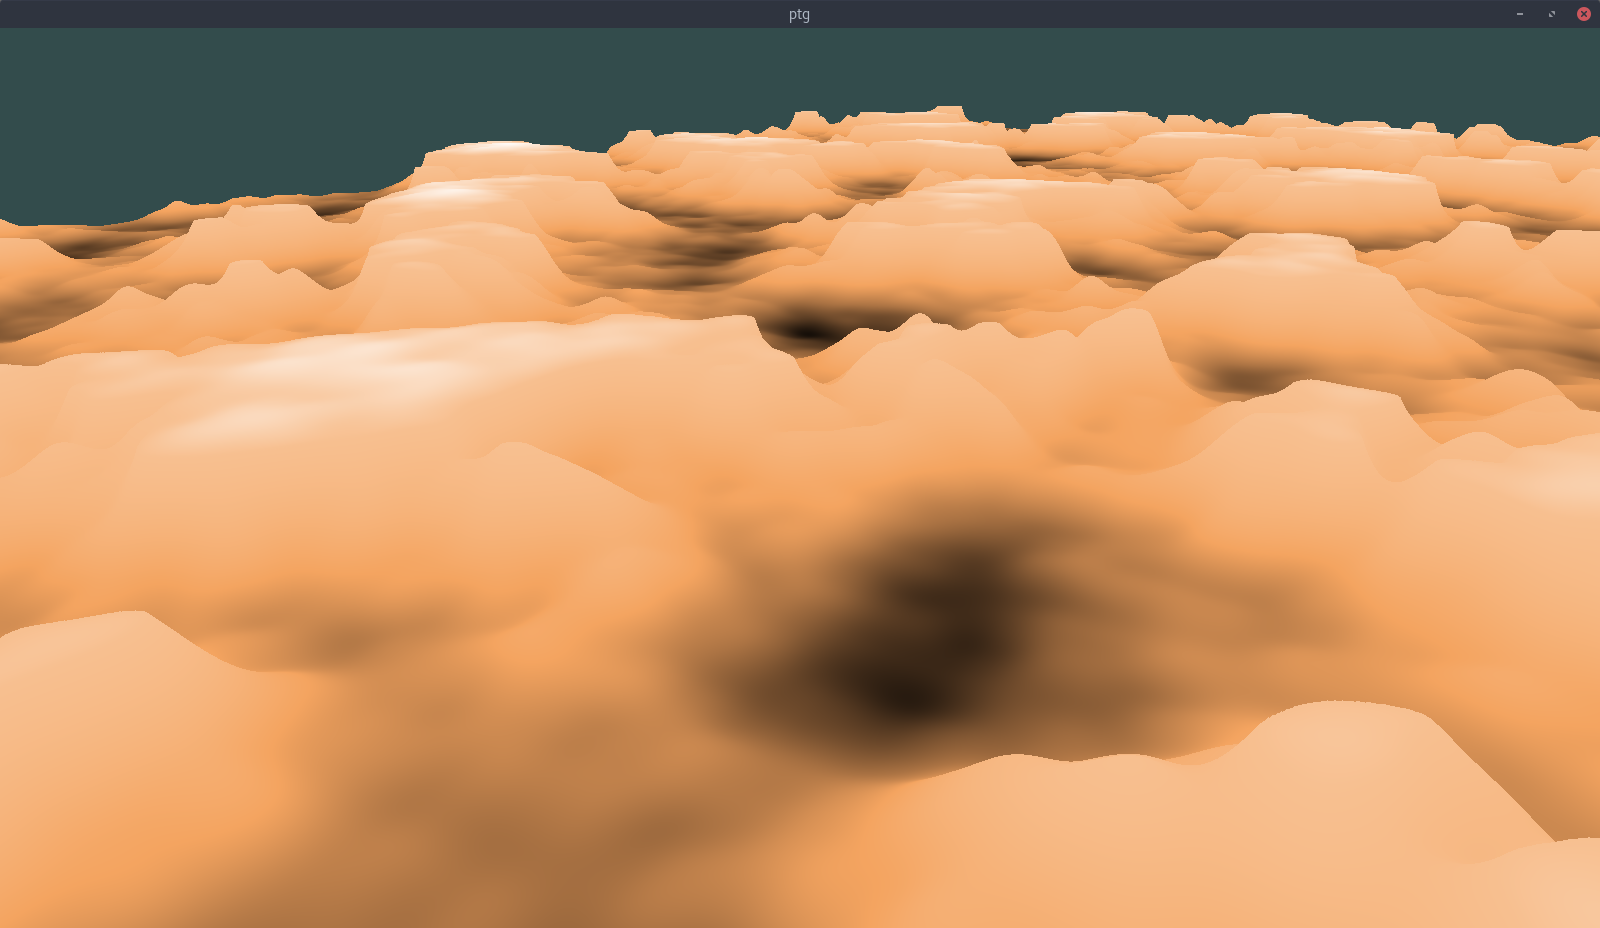
\includegraphics[width=0.5\textwidth]{figuras/bssCanyons.png}
    \caption{Consumo}
    \label{fig:bssCanyons}
\end{figure}

\section{Separando Áreas de Biomas}

\section{Detectando fronteira entre Biomas}


\setlength{\baselineskip}{\baselineskip}

%%=============================================================================
%% Referências
%%=============================================================================
%\bibliographystyle{abbrv}------------------------------------------------------Original usava essa, mas sem informações da fonte, troca para abnt
%\bibliography{referencias/referencias}
\bibliographystyle{abnt}
\bibliography{referencias/referencias}



%IMPORTANTE: Se precisar usar alguma seção ou subseção dentro dos apêndices ou
%anexos, utilizar o comando \tocless para não adicionar no Sumário
%Exemplos: 
% \tocless\section{Histórico}
%%=============================================================================
%% Apêndices
%%=============================================================================
%\appendix
%\include{capitulos/apendicea}
%\include{capitulos/apendiceb}

%%=============================================================================
%% Anexos
%%=============================================================================
%\annex
%\include{capitulos/anexoa}

\end{document}
